\documentclass{article}

\usepackage{tikz}
\usepackage{fullpage}
\usetikzlibrary{shapes.geometric,arrows}

\tikzstyle{startstop} = [rectangle, rounded corners, minimum width=3cm, minimum height=1cm,text centered, draw=black, fill=red!30]

\tikzstyle{io} = [trapezium, trapezium left angle=70, trapezium right angle=110, minimum width=3cm, minimum height=1cm, text centered, draw=black, fill=blue!30]

\tikzstyle{process} = [rectangle, minimum width=3cm, minimum height=1cm, text centered, text width=3.5cm, draw=black, fill=orange!30]

\tikzstyle{decision} = [diamond, minimum width=3cm, minimum height=1cm, text centered, text width=2cm, draw=black, fill=green!30]

\tikzstyle{arrow} = [thick,->,>=stealth]

\title{Miniopoly}

\begin{document}
\enlargethispage{8\baselineskip}
\thispagestyle{empty}
\vspace*{-2cm}
\huge{Minipoly flowchart} 
\hrule
\vspace{0.5cm}
\small
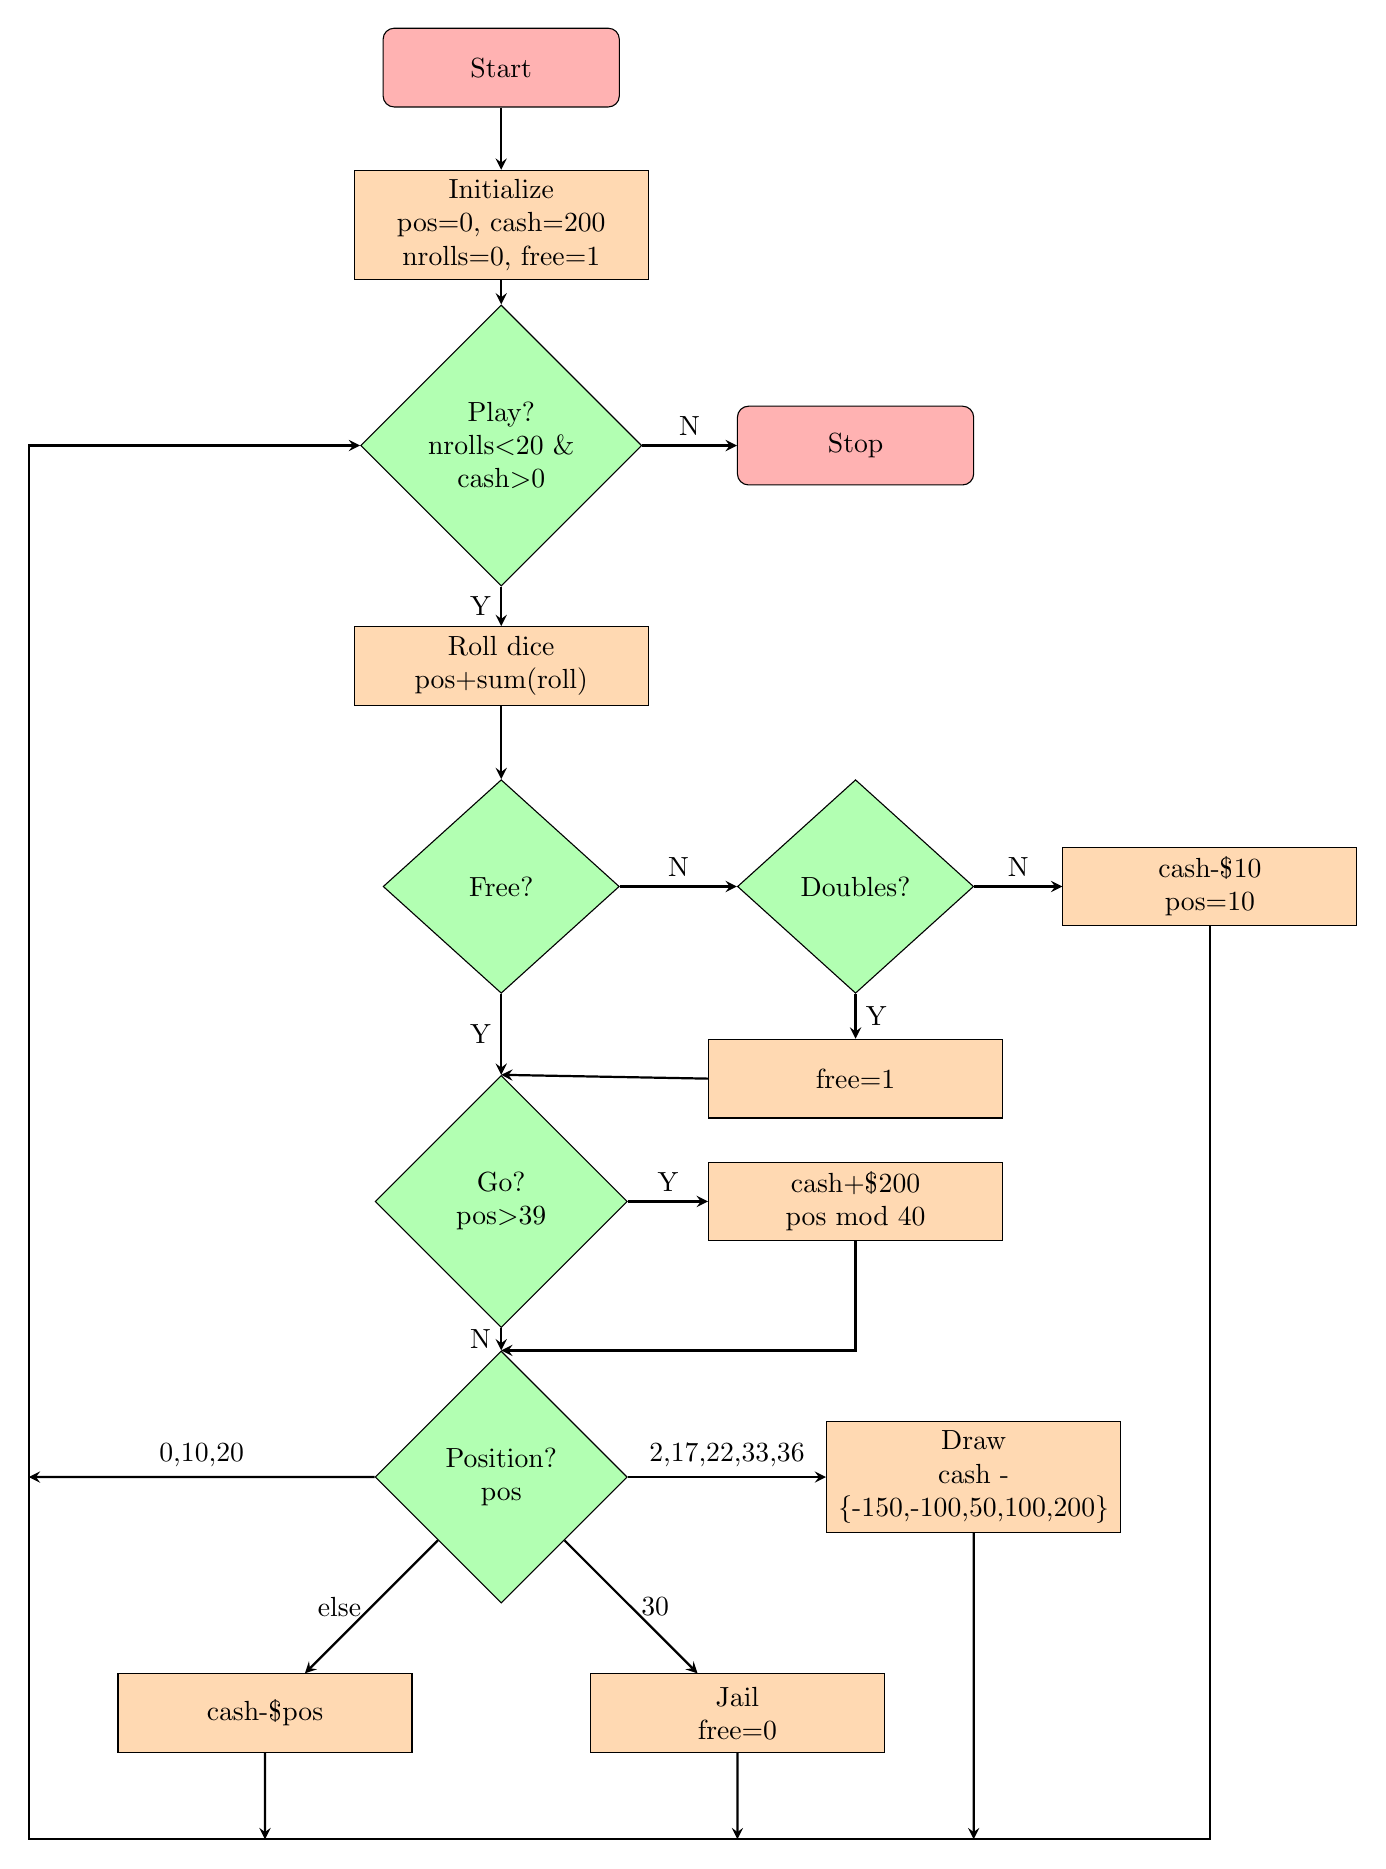
\begin{tikzpicture}[node distance=2cm]
	\node (start) [startstop] {Start};
	\node (init) [process, below of=start] {Initialize\\pos=0, cash=200\\nrolls=0, free=1};
	\node (play) [decision, below of=init, yshift=-0.8cm] {Play?\\nrolls$<$20 \&\\cash$>$0};
	\node (stop) [startstop, right of=play, xshift=2.5cm] {Stop};
	\node (roll) [process, below of=play, yshift=-0.8cm] {Roll dice\\pos+sum(roll)};
	\node (free) [decision, below of=roll, yshift=-0.8cm] {Free?};
	\node (doubles) [decision, right of=free, xshift=2.5cm] {Doubles?};
	\node (getfree) [process, below of=doubles, yshift=-0.44cm] {free=1};
	\node (pay) [process, right of=doubles, xshift=2.5cm] {cash-\$10\\pos=10};
	\node (go) [decision, below of=free, yshift=-2cm] {Go?\\pos$>$39};
	\node (200) [process, right of=go, xshift=2.5cm] {cash+\$200\\pos mod 40};
	\node (pos) [decision, below of=go, yshift=-1.5cm] {Position?\\pos};
	\node (draw) [process, right of=pos, xshift=4cm] {Draw\\ cash -\\ \{-150,-100,50,100,200\}};
	\node (jail) [process, right of=pos, xshift=1cm, yshift=-3cm] {Jail\\free=0};
	\node (paypos) [process, left of=pos, xshift=-1cm, yshift=-3cm] {cash-\$pos};
	\draw [arrow] (start) -- (init);
	\draw [arrow] (init) -- (play);
	\draw [arrow] (play) -- node[anchor=east] {Y} (roll);
	\draw [arrow] (play) -- node[anchor=south] {N} (stop);
	\draw [arrow] (roll) -- (free);
	\draw [arrow] (free) -- node[anchor=east] {Y} (go);
	\draw [arrow] (free) -- node[anchor=south] {N} (doubles);
	\draw [arrow] (doubles.south) -- node[anchor=west] {Y} (getfree);
	\draw [arrow] (doubles) -- node[anchor=south] {N} (pay);
	\draw [arrow] (getfree.west) -- (go.north);
	\draw [arrow] (go) -- node[anchor=east] {N} (pos);
	\draw [arrow] (go) -- node[anchor=south] {Y} (200);
	\draw [arrow] (200.south) |- (pos.north);
	\draw [arrow] (pos) -- node[anchor=south] {2,17,22,33,36} (draw);
	\draw [arrow] (pos) -- node[anchor=west] {30} (jail);
	\draw [arrow] (pos) -- node[anchor=east] {else} (paypos);
	\draw [arrow] (pos) -- node[anchor=south] {0,10,20} (-6,-17.9);
	\draw [arrow] (pay.south) |- (8,-22.5) -- (-6,-22.5) |- (play.west);
	\draw [arrow] (paypos.south) -- (-3,-22.5);
	\draw [arrow] (jail.south) -- (3,-22.5);
	\draw [arrow] (draw.south) -- (6, -22.5);
\end{tikzpicture}

\end{document}